\documentclass[aps,prd,amsmath,amssymb]{revtex4}


\usepackage{graphicx}
\usepackage{dcolumn}
\usepackage{bm}
\usepackage{amsmath}
\usepackage{epstopdf}
\usepackage{amsfonts}
\usepackage{amssymb}
\usepackage{epsfig}
\usepackage{tabularx}
\usepackage{color}
\usepackage{soul}
%\usepackage{hyperref}

\usepackage[colorlinks=true,citecolor=blue,urlcolor=magenta,breaklinks]{hyperref}

\newcommand{\be}{\begin{equation}}
\newcommand{\en}{\end{equation}}
\newcommand{\bea}{\begin{eqnarray}}
\newcommand{\ena}{\end{eqnarray}}

\newcommand{\dx}{ \dot{x} }
\newcommand{\dg}{ \dot{g} }
\newcommand{\ddx}{ \ddot{x} }
\newcommand{\ddg}{ \ddot{g} }
\newcommand{\dl}{ \dot{\lambda} }
\newcommand{\Wr}{ \Omega_r }
\newcommand{\Wm}{ \Omega_m }
\newcommand{\Wl}{ \Omega_\Lambda }

\newcommand{\km}{ \text{ km}}
\newcommand{\s}{ \text{ s}}
\newcommand{\Mpc}{ \text{ Mpc}}
\newcommand{\yr}{ \text{ yr}}
\newcommand{\Gyr}{ \text{ Gyr}}
\newcommand{\pc}{ \text{ pc}}
\newcommand{\LCDM}{ \Lambda\text{CDM}}

\newcommand{\newtext}[1]{{\color{red} #1}}



\begin{document}


\title{On the correlation between growth index, current cosmic acceleration \\ and Pad{\'e} dark energy parameterizations}


\author{
G. Panotopoulos,{${}^{a,b}$
\footnote{
\href{mailto:grigorios.panotopoulos@tecnico.ulisboa.pt}{grigorios.panotopoulos@tecnico.ulisboa.pt}
}
G. Barnert,{${}^{c}$
\footnote{
\href{mailto:gerald-barnert@hotmail.com}{gerald-barnert@hotmail.com} 
}
}
L. Campusano {${}^{c}$
\footnote{
\href{mailto:luis@das.uchile.cl}{luis@das.uchile.cl} 
}
}
}
}


\address{
${}^a$ Centro de Astrof{\'i}sica e Gravita{\c c}{\~a}o-CENTRA, Instituto Superior T{\'e}cnico-IST, Universidade 
de Lisboa-UL, Av. Rovisco Pais, 1049-001 Lisboa, Portugal. \\
${}^b$ Departamento de Ciencias F{\'i}sicas, Universidad de la Frontera, Avenida Francisco Salazar, Temuco 01145, Chile. \\
${}^c$ Departamento de Astronom{\'i}a, FCFM, Universidad de Chile, Camino El Observatorio 1515, Las Condes, 
Santiago, Chile.
}



\begin{abstract}
We study dynamical dark energy models within Einstein's theory by means of matter perturbations and the growth 
index $\gamma$. Contrary to the common approach, here we start assuming a linear ansatz for the growth index, and we investigate its impact on the deceleration parameter as well as the dark energy equation-of-state parameter.
We find that for viable models, $w(z)$ crosses the -1 line (quintom) ending at a present day value $w_0 > -1$. 
Furthermore, we show that an analytic expression for the dark energy equation-of-state parameter may be obtained in 
the form of (4,4) Pad{\'e} parameterizations.
\end{abstract}


\maketitle



%%%%%%%%%%%%%%%%%%%%%%%%%%%%%%%%%%%%%
\section{Introduction}\label{Intro}
%%%%%%%%%%%%%%%%%%%%%%%%%%%%%%%%%%%%%

The origin and nature of dark energy (DE), the fluid component that currently accelerates the Universe \cite{SN1,SN2,turner}, is one of the biggest mysteries and challenges in modern theoretical Cosmology. It is well-known 
that according to the cosmological equations within Einstein's General Relativity \cite{GR}, a Universe consisting of radiation and non-relativistic matter only cannot expand at an accelerating rate. On the contrary, a non-vanishing (and positive) cosmological constant \cite{einstein,carroll} has been proven to be the most economical model in an overall excellent agreement with a wealth of available observational data.

\smallskip

The $\Lambda$CDM model, based on collisionless dark matter and a positive cosmological constant, despite its success, does not come without problems. In modern times the community is facing a couple of puzzles related on the one hand to the cosmological constant problem \cite{zeldovich,weinberg} and on the other hand to the Hubble tension. To be more precise, regarding the value of the Hubble constant $H_0$, there is nowadays a disagreement between high red-shift CMB data and local measurements at low red-shift data, see e.g. \cite{tension,tension1,tension2,tension3}. The value of the Hubble constant determined by the PLANCK Collaboration \cite{planck1,planck2}, $H_0 = (67-68)~\text{km/(Mpc  sec)}$, is found to be lower than the value obtained by local measurements, $H_0 = (73-74)~\text{km/(Mpc sec)}$ \cite{hubble,recent}. This disagreement  might call for new physics \cite{newphysics,earlyDE,ben}.

\smallskip

As originally discussed by Schutz \cite{sirens}, inspiralling compact neutron star or black hole binaries are excellent standard sirens, in that their gravitational wave measurements could determine the sources’ absolute distances. 
Moreover, recent observations have accumulated compelling evidence that some short gamma-ray bursts
are associated with the mergers of neutron star binaries \cite{Ref1}. Hence, simultaneous observations of the inspiral gravitational waves and signatures in the electromagnetic band may allow us to directly and independently determine both 
the luminosity distance and red-shift to a binary \cite{Ref1}. Furthermore, adopting a second order Taylor expansion for 
the luminosity distance as a function of red-shift, $d_L(z)$ \cite{hubble,Ref2} 
\begin{equation}
d_L(z) \approx \frac{z}{H_0} \: \left[ 1+\frac{z}{2} (1-q_0) \right]
\end{equation}
a simultaneous determination of both the luminosity distance and red-shift would allow an independent determination of the Hubble constant $H_0$ \cite{Abbott}, and at the same time a measurement of $q_0$ \cite{Ref2}.


\smallskip

Due to the problems related to the cosmological constant, as was to be expected a plethora of several different 
dark energy models have been proposed and studied over the years as possible alternatives to the $\Lambda$CDM model. 
Quite generically, all dark energy models are classified into two broad classes. On the one hand, there is a family of models related to alternative/modified theories of gravity, where new correction terms appear to GR at cosmological scales. And on the other hand, in another family of models, we introduce a new dynamical field with an equation-of-state (EoS) parameter $w < -1/3$. In the first class of models, called geometrical DE, one finds for instance $f(R)$ theories of gravity \cite{mod1,mod2,HS,starobinsky}, brane-world models \cite{langlois,maartens,dgp} and Scalar-Tensor theories of gravity \cite{BD1,BD2,leandros,PR}, while in the second class, called dynamical DE, one finds models such as quintessence \cite{DE1}, phantom \cite{DE2,DE3}, quintom \cite{DE4,DE5}, tachyonic \cite{DE6} or k-essence \cite{DE7}. For an excellent 
review on the dynamics of dark energy see e.g. \cite{copeland}. 

\smallskip

Depending on the details of the underlying theory of gravity and/or the properties of the assumed DE model, the evolution
of linear matter perturbations may be affected in several different ways. Even if two DE models give the same late-time accelerating expansion, they still may differ in the matter perturbations they produce \cite{staro,radouane}. This fact
could provide an additional important way to discriminate between various models
(see e.g. \cite{extra1,extra2,extra3,extra4}). It is therefore important to characterize as accurately as possible the growth of matter perturbations. An important issue is to characterize departures at low red-shift for different
models. A quantity that has been studied a lot over the years is the so called growth index $\gamma$ introduced in \cite{gamma}. 

\smallskip

In the present work we propose to study the correlation between a linear ansatz for the growth index, and the deceleration parameter and the DE equation-of-state parameter. Contrary to the common approach in which one first assumes a concrete DE model and then solves the equation for the matter density contrast to compute the growth index, here we propose to follow the inverse approach, namely we shall first assume a linear ansatz for the growth index and we shall investigate its impact
on properties of dark energy.

\smallskip

Our plan in the present article is the following: After this introduction, in the next section we briefly review the 
standard Friedmann-Robertson-Walker Universe at background level as well as the linear cosmological perturbations. In section 3 we show and discuss our main numerical results. Finally, we close our work with some concluding remarks in the last section. We adopt the mostly positive metric signature, $(-,+,+,+)$, and we work in units where the speed of light in vacuum is set to unity, $c=1$.



%%%%%%%%%%%%%%%%%%%%%%%%%%%%%%%%%
\section{Theoretical framework}
%%%%%%%%%%%%%%%%%%%%%%%%%%%%%%%%%

The starting point is Einstein's GR \cite{GR} based on the Einstein-Hilbert term coupled to the matter content
\begin{equation}
S = \int d^4x \sqrt{-g} \left[ \frac{R}{16 \pi G}  + \mathcal{L}_M \right]
\end{equation}
where $g_{\mu \nu}$ is the metric tensor, $g$ is its determinant, $R$ is the corresponding Ricci scalar, $G$ is Newton's constant and $\mathcal{L}_M$ is the Lagrangian of the matter content. Varying the action with respect to the metric tensor
one obtains the well-known Einstein's field equations, which read
\begin{equation}
G_{\mu \nu} \equiv R_{\mu \nu} - \frac{1}{2} R g_{\mu \nu} = 8 \pi G \: T_{\mu \nu}
\end{equation}
where $R_{\mu \nu}$ is the Ricci tensor, while $T_{\mu \nu}$ is the matter energy-momentum tensor.


\subsection{Background evolution}

The basic cosmological equations governing the expansion of a homogeneous and isotropic Universe may be found e.g. in
\cite{review}. If matter consists of a perfect fluid with pressure $p$ and energy density $\rho$, the energy momentum 
tensor is given by
\begin{equation}
T_{\mu \nu} = p \: g_{\mu \nu} + (p + \rho) \: u_\mu \: u_\nu 
\end{equation}
where $u_\mu$ is the four-velocity of the fluid satisfying the condition $u_\mu u^\mu = -1$. The mixed component
stress-energy tensor takes the form \cite{review}
\begin{equation}
T_{\nu}^{\mu} =\textrm{diag}(-\rho,p,p,p)
\end{equation}

A spatially flat, isotropic and homogeneous universe is described by a Robertson-Walker metric \cite{review}
\begin{equation}
ds^2 = -dt^2 + a(t)^2 \delta_{ij} dx^i dx^j 
\end{equation}
where the scale factor $a(t)$ is the only unknown quantity, and all quantities depend on the cosmic time $t$ only.

\smallskip

The cosmological equations are found to be the continuity equation as well as the two Friedmann
equations \cite{review}
\begin{eqnarray}
H^2 & = & \frac{8 \pi G}{3} \rho \\
\frac{\ddot{a}}{a} & = & -\frac{4 \pi G}{3} (\rho + 3p) \\
0 & = & \dot{\rho} + 3 H (\rho+p)
\end{eqnarray}
where an over dot denotes differentiation with respect to cosmic time, and $H=\dot{a}/a$ is the Hubble parameter. The
second Friedmann equation may be written down equivalently as follows
\begin{equation}
\dot{H} = \frac{\ddot{a}}{a} - H^2 = - 4 \pi G (\rho+p)
\end{equation}
Finally, the deceleration parameter, $q$, is defined by
\begin{equation}
q \equiv - \frac{\ddot{a}}{aH^2}
\end{equation}
and as a function of red-shift, $z=-1+a_0/a$, with $a_0$ being the present value of the scale factor, it is computed to be
\begin{equation}
q(z) = -1 + (1+z) \frac{H'(z)}{H(z)}
\end{equation}
In the following, instead of the cosmic time, $t$, we shall be using either the scale factor, $a$, or the red-shift, 
$z$, as the independent variable.

\smallskip

If there are several non-interacting fluid components, then
\begin{eqnarray}
p & = & \sum_i p_i \\
\rho & = & \sum_i \rho_i \\
0 & = & \dot{\rho_i} + 3 H (\rho_i+p_i)
\end{eqnarray}
For barotropic fluids $p=w \rho$, where $w$ is the equation-of-state parameter. Finally, it is convenient to
introduce for each fluid component $X$ the normalized (dimensionless) density, $\Omega_X$, which is defined to be
\begin{align}
\Omega_X &\equiv \frac{\rho_{X}}{\rho_{c}}\,, \quad \rho_c=\frac{3H_0^2}{8 \pi G}\,,
\end{align}
with $H_0$ being the Hubble parameter evaluated at today. The normalized density as a function of the scale factor 
takes the form
\begin{equation}
\Omega_X(a) = \frac{\Omega_{X,0}}{a^3 E(a)^2}
\end{equation}
where $\Omega_{X,0}$ is the normalized density of the $X$ component evaluated at today, while the dimensionless expansion
history, $E(a)$, is given by 
\begin{align}
E(a)^2 \equiv \left(\frac{H(a)}{H_0}\right)^2 = \Omega_m a^{-3} + (1 - \Omega_m) F(a)
\end{align}
neglecting radiation at low red-shift, $1+z=a_0/a$, of order one or so, where $F(a)$ is determined by the DE 
equation-of-state parameter as follows
\begin{equation}
w(z) = -1 + (1+z) \: \frac{F'(z)}{3 F(z)}.
\end{equation}
Clearly, the present value values of both $E(a)$ and $F(a)$ equal to unity
\begin{equation}
E(a=1) = 1, \; \; \; \; \; F(a=1) = 1.
\end{equation}



\subsection{Linear cosmological perturbations}

Let us briefly review linear cosmological perturbation theory within GR, see e.g. \cite{Mukhanov:2005sc,other}.

\smallskip

The goal is to solve the perturbed Einstein's field equations
\begin{equation}
\delta G_\nu^\mu = 8 \pi G \: \delta T_\nu^\mu
\end{equation}
On the one hand, for scalar perturbations relevant in growth of structures, the metric tensor has the form
\begin{equation}
ds^2 = -(1 + 2 \Psi) dt^2 + (1-2 \Psi) \delta_{ij} dx^i dx^j
\end{equation}
where $\Psi$ is the metric perturbation, while for the cosmological fluid the perturbed stress-energy tensor has the form
\begin{equation}
\delta T_0^0 = \delta \rho, \qquad \delta T_j^i = - \delta p \: \delta_j^i
\end{equation}
The full set of coupled equations for matter and metric perturbations may be found e.g. in \cite{mariam,pano1,pano2}.

\smallskip

The Fourier transform of the density contrast, $\delta_k = \delta \rho_m / \rho_m$, with $k$ being the wave number,
for pressure-less matter satisfies the following linear differential equation \cite{rogerio,leandros2,review2}
\begin{equation}
\ddot{\delta_k} + 2H \dot{\delta_k} - 4 \pi G \rho_m \delta_k = 0
\end{equation}
at linear level assuming that DE does not cluster (homogeneous DE), $\delta_k \ll 1$, and for sub-horizon 
scales, $k/(2 \pi a) \gg a H$, when only non-relativistic matter clusters. During matter domination
\begin{equation}
a(t) \sim t^{2/3}, \; \; \; \; \; H(t) = \frac{2}{3 t}
\end{equation}
the matter density contrast  grows linearly with the scale factor, $\delta_k(a) \sim a$.

\smallskip

The equation for $\delta$ may be take equivalently the following form 
%
\begin{align}
\delta''(a) + \left( \frac{3}{a} + \frac{E'(a)}{E(a)} \right) \delta'(a) - \frac{3}{2} \frac{\Omega_m}{a^5 E(a)^2} \delta(a) = 0
\end{align}
%
where for simplicity we drop the sub-index $k$, a prime denotes differentiation with respect to the scale factor.

\smallskip

The growth index, $\gamma$, is defined to be
%
\begin{equation}
f \equiv \frac{d \ln \delta}{d \ln a} = \frac{a}{\delta} \: \frac{d \delta}{d a}
\end{equation}
%
\begin{equation}
f = \Omega_m^\gamma
\end{equation}
%
or equivalently
%
\begin{equation}
\gamma(a) = \frac{ln(f(a))}{ln(\Omega_m(a))}
\end{equation}
%
For a constant DE equation-of-state, $w(z)=w$, there is an impressive agreement between the numerical result and an 
analytic approximation, and we find at lowest order \cite{leandros2}
\begin{equation}
\gamma = \frac{3(w-1)}{6w-5}
\end{equation}
around $z \sim 1$. This reduces to $\gamma=6/11$ for $\Lambda$CDM ($w=-1$). In full generality, however, the growth index is a function of red-shift, with a non-vanishing derivative $\gamma'(z) \equiv d\gamma(z)/dz$. In an attempt to further improve on the analytic approximation, in \cite{radouane,leandros2} the authors considered an expansion to first order in $z$ of the form
\begin{equation}
\gamma(z) = \gamma_0 + \gamma_1 z
\end{equation}
which could have interesting observational consequences, and which is characterized by two parameters that may be identified with today's values of the functions $\gamma(z),\gamma'(z)$
\begin{equation}
\gamma_0 = \gamma(z=0), \;\;\;\;\;  \gamma_1 = \gamma'(z=0)
\end{equation}

During matter domination, since $\delta \propto a$, by definition $f$ is found to be $f(a)=1$. Furthermore, the second order differential equation for $\delta$ may be written down equivalently as a first order differential equation for $f(a)$
as follows
\begin{equation}
a f'(a) + f(a)^2 + f(a) \left( 2 + a \frac{E'(a)}{E(a)} \right) = \frac{3 \Omega_m(a)}{2}.
\end{equation}



%%%%%%%%%%%%%%%%%%%%%%%%%%%%%%
\section{Numerical results}
%%%%%%%%%%%%%%%%%%%%%%%%%%%%%%

As already mentioned before, in the present work instead of assuming a concrete DE model, i.e. a given parameterization
$w(a)$ or $w(z)$, we shall assume following \cite{radouane,leandros2} that the evolution of matter perturbations implies a linear growth index on the red-shift space of the form
\begin{equation}
\gamma(z) = \gamma_0 + \gamma_1 z
\end{equation}
valid at low red-shift in the range $0 \leq z \leq 1$. The parameters $\gamma_0,\gamma_1$ are allowed to vary in 
the range \cite{radouane}
\begin{equation}
0.5 < \gamma_0 < 0.6, \; \; \; \; \; -0.05 < \gamma_1 < 0.05
\end{equation}
and we ask ourselves the question what the impact of those two free parameters is on properties of DE, such as the equation-of-state parameter, $w(z)$, and the deceleration parameter evaluated at today, $q_0$.

\smallskip

Let us briefly describe the approach followed here. Since the DE model is a priori unknown, all quantities of interest may be expressed in terms of the unknown function $F(a)$, which is directly related to the DE equation-of-state $w(a)$. The differential equation for $f(a)$ may be viewed as a differential equation for $F(a)$ instead, subjected to the initial condition $F(a=1)=1$. Once the numerical values of 
$\Omega_{m,0},\gamma_0,\gamma_1$ are specified, the differential equation may be integrated numerically, and after that $q(z)$ and $w(z)$ may be computed in a straightforward manner. 

\smallskip

Our main numerical results are summarized in the figures below. Throughout the numerical analysis we set 
$\Omega_{m,0}=0.3$, and we vary both $\gamma_0$ and $\gamma_1$. In the left panel of Fig.~\ref{fig:1} we show
$q_0$ versus $\gamma_1$ for a given $\gamma_0$. The three different curves correspond to distinct numerical values of 
$\gamma_0=0.52,0.55,0.59$ from bottom to top. For a given $\gamma_0$ $q_0$ decreases with $\gamma_1$ almost linearly, 
while as $\gamma_0$ increases the curves are shifted upwards, and they are less rapidly varying functions of $\gamma_1$.

\smallskip

Similarly to the left panel, in the right panel of Fig.~\ref{fig:1} we show $q_0$ versus $\gamma_1$ for a fixed 
$\gamma_0=0.55$, showing at the same time the horizontal strip corresponding to the allowed range $q_0=0.05 \pm 0.08$. 
Thus, we obtain for $\gamma_1$ the constraint $-0.042 \leq \gamma_1 \leq -0.029$. For the two extreme values corresponding to the lower and upper bound of $\gamma_1$, we show in the bottom panel of Fig.~\ref{fig:1} the equation-of-state parameter
$w(z)$. In the case represented by the red curve, $w(z)$ remains always below the $-1$ line, and therefore DE is phantom \cite{DE2,DE3}. At a more fundamental level based on a Lagrangian description, this class of dynamical DE model may be analyzed introducing a real scalar field with the "wrong" sign in from of its kinetic term. On the other hand, the case represented by the blue curve crosses the $-1$ line, and therefore DE is quintom \cite{DE4,DE5}. This time at a more fundamental level based on a Lagrangian description, this class of dynamical DE model may be analyzed introducing two real scalar fields, one minimally coupled and another with the "wrong" sign in from of its kinetic term \cite{saridakis1,saridakis2}.

\smallskip

Next, the impact of the $\gamma_1$ variation on $q(z)$ (left panel) and $w(z)$ (right panel) is shown in Fig.~\ref{fig:2} setting $\gamma_0=0.55$ and $\Omega_{m,0}=0.3$. We have considered four different values of 
$\gamma_1=-0.04,-0.02,0.02,0.04$. The equation-of-state parameter crosses the $-1$ line (quintom) either from lower to higher values when $\gamma_1$ is negative or from higher to lower values when $\gamma_1$ is positive. Moreover, both $q_0$
and the transition red-shift, $z_*$, between deceleration and acceleration decrease with $\gamma_1$.

\smallskip

Finally, and before we conclude our work, a comment is in order here. Within our approach the DE equation-of-state may be obtained numerically. However, it would be both desirable and advantageous to have an analytic expression for $w(z)$. One way to do that is to fit the function $F(z)$ with a polynomial of degree $n$, $F(z) \approx P_n(z)$. Recall that $F(z)$ is directly related to $w(z)$. Then it is easy to verify that the DE equation-of-state parameter takes the form of a ($m,n$) Pad{\'e} parameterization \cite{PADE}, which quite generically for any given function $h(z)$ is given by \cite{pade1,pade2}
\begin{equation}
h(z) = \frac{R_n(z)}{Q_m(z)} = \frac{c_0+c_1 z + ... + c_n z^n}{d_0+d_1 z + ... + d_m z^m}
\end{equation}
namely it is a rational function where both the numerator and the denominator are polynomials of degree $n$ and $m$, respectively. To check if the fit is a good one, we compute the relative error with respect the real numerical solution, and we require that it is not higher than $5 \%$. We have carefully checked that low degree polynomials are not acceptable according to our criterion, and that the Pad{\'e} approximation for the DE EoS parameter must be at least (4,4). For instance, in the case where $\Omega_{m,0}=0.3, \gamma_0=0.55$ and $\gamma_1=-0.029$, we found the following analytic expression for $w(z)$
\begin{eqnarray}
w(z) & = & \frac{R_4(z)}{Q_4(z)}, \\
R_4(z) & = & 0.33 z^4+1.33 z^3-1.98 z^2-0.03 z-3.25, \\
Q_4(z) & = & z^4-2.08 z^3-0.29 z^2-0.25 z+3.17,
\end{eqnarray}
while in the case where $\Omega_{m,0}=0.3, \gamma_0=0.55$ and $\gamma_1=-0.042$, we found the following analytic expression for $w(z)$
\begin{eqnarray}
w(z) & = & \frac{R_5(z)}{Q_5(z)}, \\
R_5(z) & = & 0.65 z^5 + 1.34 z^4-1.29 z^3 +0.09 z^2-1.37 z-1.32, \\
Q_4(z) & = & z^5 -0.97 z^4-0.4 z^3-1.46 z^2 + 0.59 z + 1.52.
\end{eqnarray}


%%%%%%%%%%%%%%%%%%%%%%%%%%%%%%BEGIN-FIGURES%%%%%%%%%%%%%%%%%%%%%%%%%%%%%%%%

\begin{figure*}[ht]
\centering
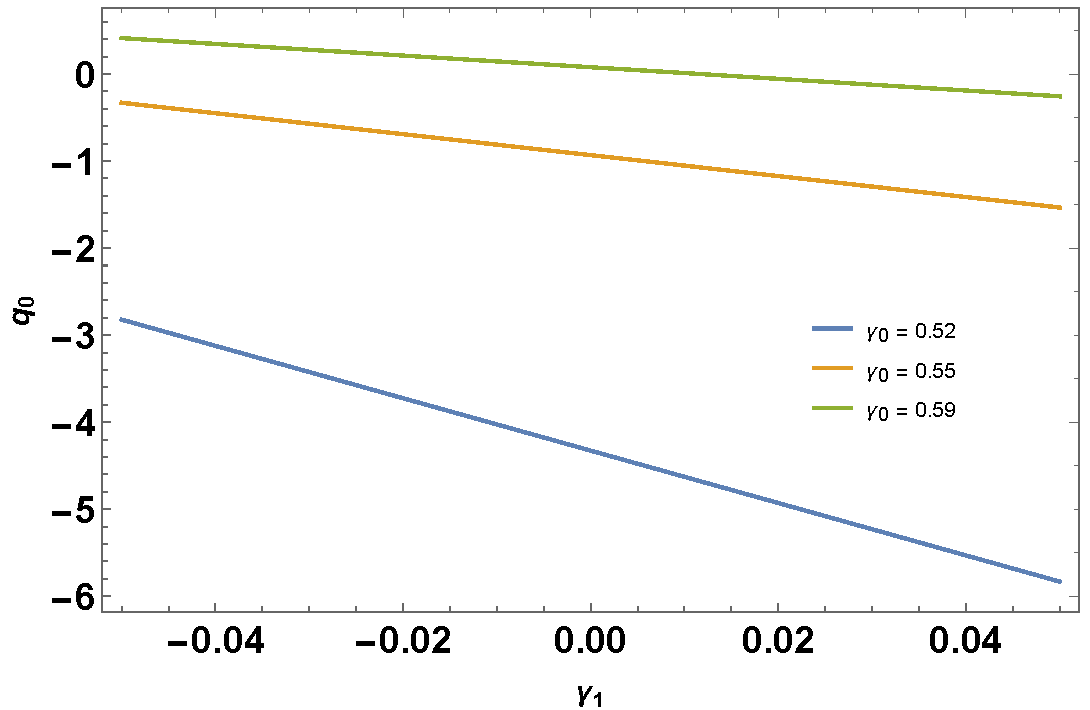
\includegraphics[width=0.4\textwidth]{q0VSgamma1.pdf}   \
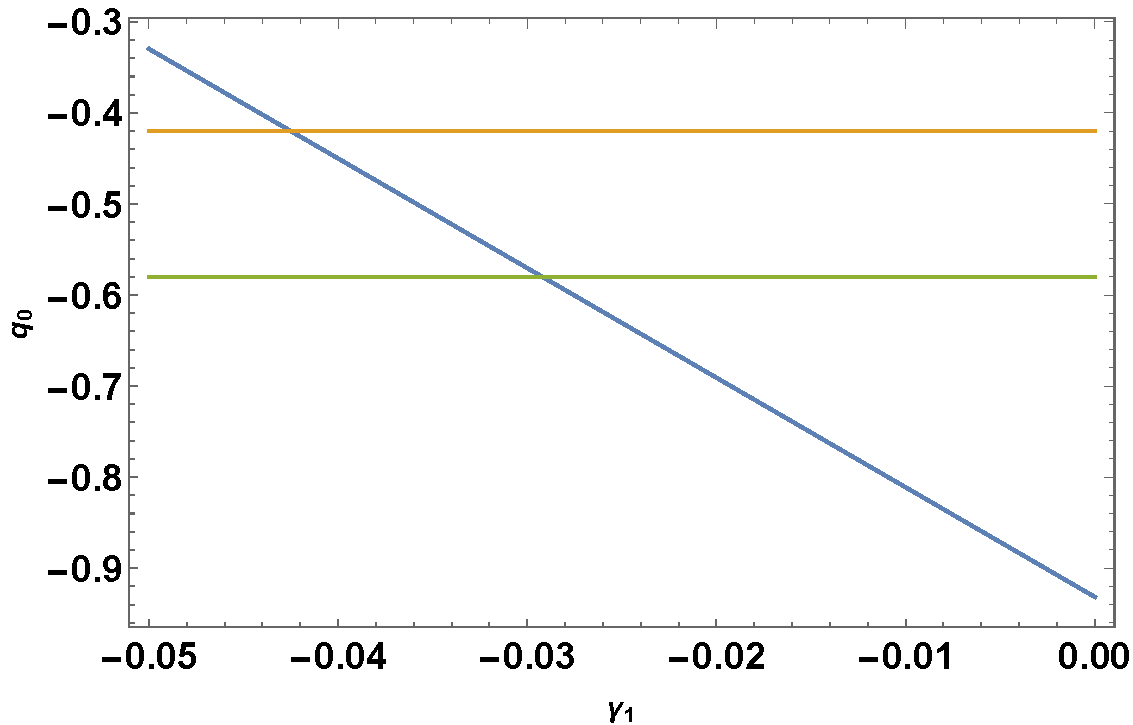
\includegraphics[width=0.4\textwidth]{Bounds.pdf}   \
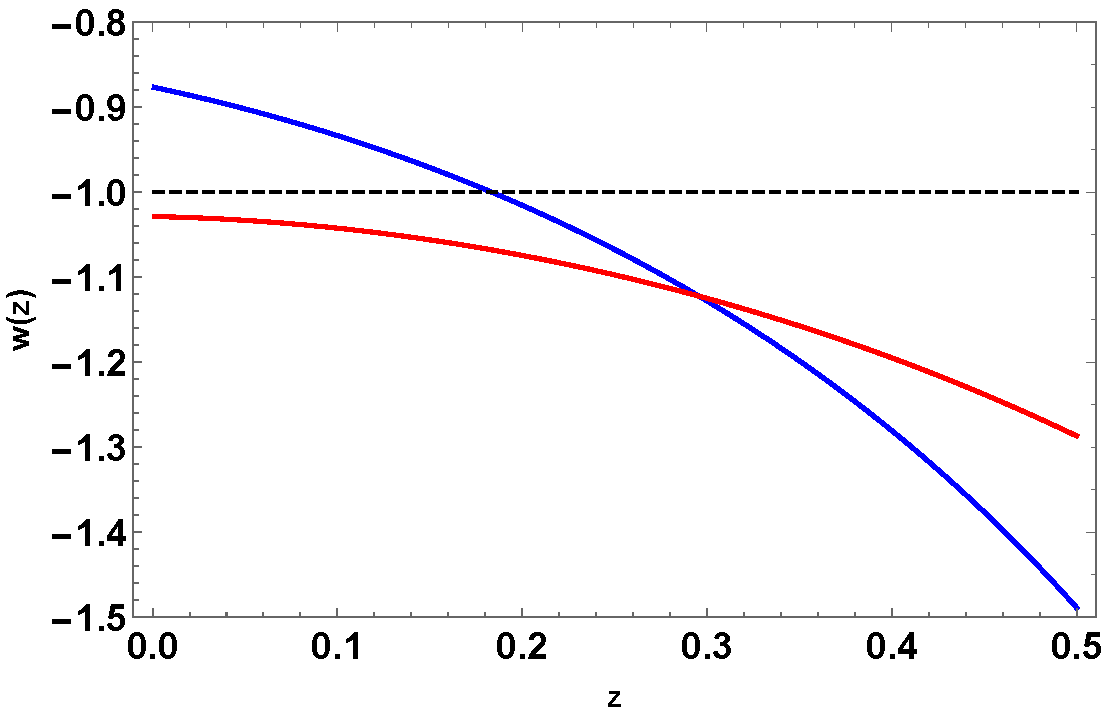
\includegraphics[width=0.4\textwidth]{wVSz_Extremes}   \
\caption{
{\bf Top left:} Deceleration parameter evaluated at today, $q_0$, versus $\gamma_1$ for $\Omega_{m,0}=0.3$ and $\gamma_0=0.52,0.55,0.59$.
{\bf Top right:} $q_0$ versus $\gamma_1$ for $\Omega_{m,0}=0.3$ and $\gamma_0=0.55$. The limits $q_0=0.5 \pm 0.08$
are shown as well.
{\bf Bottom:} Equation-of-state parameter, $w$, versus red-shift, $z$, for $\Omega_{m,0}=0.3, \gamma_0=0.55$ and 
$\gamma_1=-0.042$ (blue color) and $\gamma_1=-0.029$ (red color).
}
\label{fig:1}
\end{figure*}

%%%%%%%%%%%%%%%%%%%%%%%%%%%%%%%%%%%%%%%%%%%%%%%%%%%%%

\begin{figure}
\centering
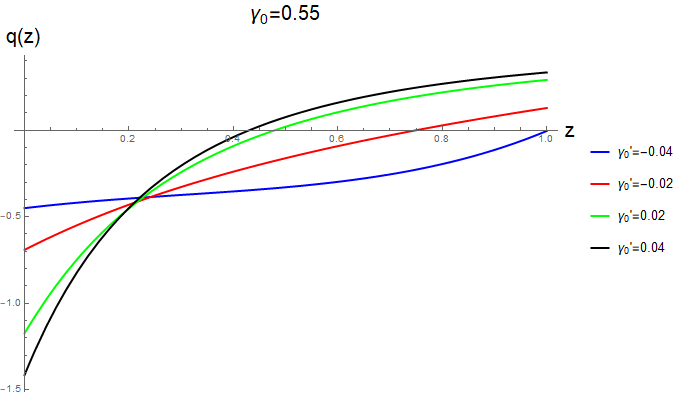
\includegraphics[width=0.4\linewidth]{q_gamma055.png} \
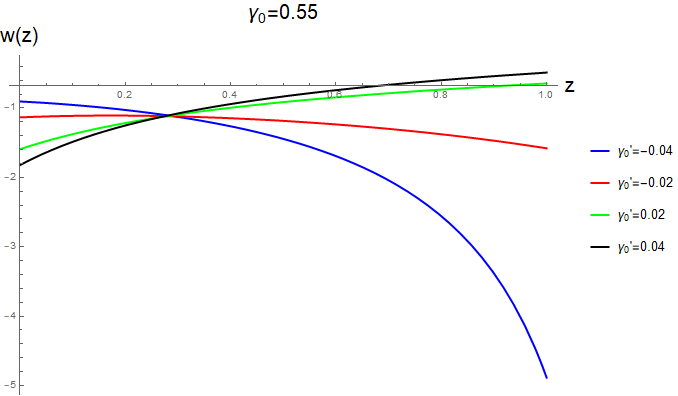
\includegraphics[width=0.4\linewidth]{w_gamma055.png} \
\caption{
{\bf Left:} Deceleration parameter, $q$, versus red-shift, $z$, for $\Omega_{m,0}=0.3, \gamma_0=0.55$ and 
$\gamma_1=-0.04 ,-0.02, 0.02, 0.04$.
{\bf Right:} Equation-of-state parameter, $w$, versus red-shift, $z$, for $\Omega_{m,0}=0.3, \gamma_0=0.55$ and 
$\gamma_1=-0.04, -0.02, 0.02, 0.04$.
}
\label{fig:2}
\end{figure}


%%%%%%%%%%%%%%%%%%%%%%%%%%%END-FIGURES%%%%%%%%%%%%%%%%%%%%%%%%%%%%%%%%%%%%%



%%%%%%%%%%%%%%%%%%%%%%
\section{Conclusions}
%%%%%%%%%%%%%%%%%%%%%%%

In summary, the present work has been devoted to the study of dynamical DE models within 4D GR.
Assuming that DE does not cluster, the starting point was the differential equation for the density
contrast of non-relativistic matter. Instead of the usual treatment where one assumes a certain
DE model and computes the growth index, here we followed the inverse approach. To be more precise,
we first assumed for $\gamma(z)$ a linear ansatz $\gamma(z)=\gamma_0+\gamma_1 z$ valid at low red-shift, 
$0 < z < 1$, and we asked ourselves the question what its impact would be on the properties of DE. Our main 
numerical results show that for fixed $\Omega_{m,0}, \gamma_0$, $q_0$ is a decreasing function of $\gamma_1$, whereas
for a given $\gamma_1$, the curves are shifted upwards as $\gamma_0$ increases. Furthermore, for
viable models it has been found that $w(z)$ crosses the -1 line from very negative values initially (phantom), 
ending at a present day value $w_0 > -1$ (quintessence). This behavior, called quintom in the literature,
may be obtained at the level of a Lagrangian description introducing two real scalar fields, one of which enters
with the wrong sign in front of the kinetic term. Finally, we have shown that an analytic expression for the 
DE equation-of-state parameter may be obtained in the form of Pad{\'e} DE parameterizations, and that the 
order of the Pad{\'e} approximation must be at least (4,4).



%%%%%%%%%%%%%%%%%%%%%%%%%%%%%%%%%%%%%%%%%%%%%%%%%%%%%%%%%%%%%%%%%%%%%%%%%%%

\section*{Acknowlegements}

The author G.~P. thanks the Fun\-da\c c\~ao para a Ci\^encia e Tecnologia (FCT), Portugal, 
for the financial support to the Center for Astrophysics and Gravitation-CENTRA, Instituto 
Superior T\'ecnico, Universidade de Lisboa, through the Grants No. UID/FIS/00099/2013 and 
No. PTDC/FIS-AST/28920/2017. 

%%%%%%%%%%%%%%%%%%%%%%%%%%%%%%%%%%%%%%%%%%%%%%%%%%%%%%%%%%%%%%%%%%%%%%%%%%%%%%%%%%


\begin{thebibliography}{99}
%
\bibitem{SN1} A.~G.~Riess et al. Astron. J. 116, 1009 (1998).

\bibitem{SN2} S.~Perlmutter et al., Astrophys. J. 517, 565 (1999).

\bibitem{turner} W.~L.~Freedman and M.~S.~Turner,
%``Measuring and understanding the universe,''
  Rev.\ Mod.\ Phys.\  {\bf 75} (2003) 1433
[astro-ph/0308418].

\bibitem{GR} A.~Einstein, 
  % "The Foundation of the General Theory of Relativity," 
Annalen Phys. 49 (1916) 769–822.

\bibitem{einstein} A.~Einstein,
  %``Cosmological Considerations in the General Theory of Relativity,''
  Sitzungsber.\ Preuss.\ Akad.\ Wiss.\ Berlin (Math.\ Phys.\ ) {\bf 1917} (1917) 142.
  
\bibitem{carroll} S.~M.~Carroll,
  %``The Cosmological constant,''
  Living Rev.\ Rel.\  {\bf 4} (2001) 1
%  doi:10.12942/lrr-2001-1
  [astro-ph/0004075].

\bibitem{weinberg} S.~Weinberg,
  %``The Cosmological Constant Problem,''
  Rev.\ Mod.\ Phys.\  {\bf 61} (1989) 1.
  
\bibitem{zeldovich} Y.~B.~Zeldovich,
  %``Cosmological Constant and Elementary Particles,''
  JETP Lett.\  {\bf 6} (1967) 316
  [Pisma Zh.\ Eksp.\ Teor.\ Fiz.\  {\bf 6} (1967) 883].


\bibitem{tension} B.~Ryden,
  %``A constant conflict,''
  Nature Phys.\  {\bf 13} (2017) no.3,  314.

\bibitem{tension1} L.~Verde, P.~Protopapas and R.~Jimenez,
  %``Planck and the local Universe: Quantifying the tension,''
  Phys.\ Dark Univ.\  {\bf 2} (2013) 166
  [arXiv:1306.6766 [astro-ph.CO]].

\bibitem{tension2} K.~Bolejko,
  %``Emerging spatial curvature can resolve the tension between high-redshift CMB and low-redshift distance ladder measurements of the Hubble constant,''
  Phys.\ Rev.\ D {\bf 97} (2018) no.10,  103529
 % [arXiv:1712.02967 [astro-ph.CO]].

\bibitem{tension3} E.~Mörtsell and S.~Dhawan,
  %``Does the Hubble constant tension call for new physics?,''
  arXiv:1801.07260 [astro-ph.CO].
  
\bibitem{planck1} P.~A.~R.~Ade {\it et al.} [Planck Collaboration],
  %``Planck 2015 results. XIII. Cosmological parameters,''
  Astron.\ Astrophys.\  {\bf 594} (2016) A13
  [arXiv:1502.01589 [astro-ph.CO]].
  
\bibitem{planck2} N.~Aghanim {\it et al.} [Planck Collaboration],
  %``Planck 2018 results. VI. Cosmological parameters,''
  arXiv:1807.06209 [astro-ph.CO].
  
\bibitem{hubble} A.~G.~Riess {\it et al.},
  %``A 2.4% Determination of the Local Value of the Hubble Constant,''
  Astrophys.\ J.\  {\bf 826} (2016) no.1,  56
  [arXiv:1604.01424 [astro-ph.CO]].
  
\bibitem{recent} A.~G.~Riess {\it et al.},
  %``Milky Way Cepheid Standards for Measuring Cosmic Distances and Application to Gaia DR2: Implications for the Hubble Constant,''
  Astrophys.\ J.\  {\bf 861} (2018) no.2,  126
  [arXiv:1804.10655 [astro-ph.CO]].  

\bibitem{newphysics} E.~M{\"o}rtsell and S.~Dhawan,
  %``Does the Hubble constant tension call for new physics?,''
  JCAP {\bf 1809} (2018) no.09,  025
%  doi:10.1088/1475-7516/2018/09/025
  [arXiv:1801.07260 [astro-ph.CO]].
  
\bibitem{earlyDE} V.~Poulin, T.~L.~Smith, T.~Karwal and M.~Kamionkowski,
%``Early Dark Energy Can Resolve The Hubble Tension,''
Phys. Rev. Lett. \textbf{122} (2019) no.22, 221301
%doi:10.1103/PhysRevLett.122.221301
[arXiv:1811.04083 [astro-ph.CO]].
  
\bibitem{ben} P.~D.~Alvarez, B.~Koch, C.~Laporte and \'A.~Rinc\'on,
%``Can scale-dependent cosmology alleviate the $H_0$ tension?,''
JCAP \textbf{06} (2021), 019
%doi:10.1088/1475-7516/2021/06/019
[arXiv:2009.02311 [gr-qc]].  
  
\bibitem{sirens} Schutz, B. F. 1986, Nature, 323, 310.  

\bibitem{Ref1} S.~Nissanke, D.~E.~Holz, N.~Dalal, S.~A.~Hughes, J.~L.~Sievers and C.~M.~Hirata,
%``Determining the Hubble constant from gravitational wave observations of merging compact binaries,''
[arXiv:1307.2638 [astro-ph.CO]].

\bibitem{Ref2} S.~M.~Feeney, H.~V.~Peiris, A.~R.~Williamson, S.~M.~Nissanke, D.~J.~Mortlock, J.~Alsing and D.~Scolnic,
%``Prospects for resolving the Hubble constant tension with standard sirens,''
Phys. Rev. Lett. \textbf{122} (2019) no.6, 061105
%doi:10.1103/PhysRevLett.122.061105
[arXiv:1802.03404 [astro-ph.CO]].

\bibitem{Abbott} B.~P.~Abbott \textit{et al.} [LIGO Scientific, Virgo, 1M2H, Dark Energy Camera GW-E, DES, DLT40, Las Cumbres Observatory, VINROUGE and MASTER],
%``A gravitational-wave standard siren measurement of the Hubble constant,''
Nature \textbf{551} (2017) no.7678, 85-88
%doi:10.1038/nature24471
[arXiv:1710.05835 [astro-ph.CO]].
  
\bibitem{mod1} T.~P.~Sotiriou and V.~Faraoni,
  %``f(R) Theories Of Gravity,''
  Rev.\ Mod.\ Phys.\  {\bf 82} (2010) 451
  [arXiv:0805.1726 [gr-qc]].

\bibitem{mod2} A.~De Felice and S.~Tsujikawa,
  %``f(R) theories,''
  Living Rev.\ Rel.\  {\bf 13} (2010) 3
  [arXiv:1002.4928 [gr-qc]].

\bibitem{HS} W.~Hu and I.~Sawicki,
  %``Models of f(R) Cosmic Acceleration that Evade Solar-System Tests,''
  Phys.\ Rev.\ D {\bf 76} (2007) 064004
  [arXiv:0705.1158 [astro-ph]].

\bibitem{starobinsky} A.~A.~Starobinsky,
  %``Disappearing cosmological constant in f(R) gravity,''
  JETP Lett.\  {\bf 86} (2007) 157
 %[arXiv:0706.2041 [astro-ph]].
 
\bibitem{langlois} D.~Langlois,
  %``Brane cosmology: An Introduction,''
  Prog.\ Theor.\ Phys.\ Suppl.\  {\bf 148} (2003) 181
  [hep-th/0209261].

\bibitem{maartens} R.~Maartens,
  %``Brane world gravity,''
  Living Rev.\ Rel.\  {\bf 7} (2004) 7
  [gr-qc/0312059].

\bibitem{dgp} G.~R.~Dvali, G.~Gabadadze and M.~Porrati,
  %``4-D gravity on a brane in 5-D Minkowski space,''
  Phys.\ Lett.\ B {\bf 485} (2000) 208
[hep-th/0005016].

\bibitem{BD1} C.~Brans and R.~H.~Dicke,
  %``Mach's principle and a relativistic theory of gravitation,''
  Phys.\ Rev.\  {\bf 124} (1961) 925.
  
\bibitem{BD2} C.~H.~Brans,
  %``Mach's Principle and a Relativistic Theory of Gravitation. II,''
  Phys.\ Rev.\  {\bf 125}, 2194 (1962).
  
\bibitem{leandros} J.~C.~B.~Sanchez and L.~Perivolaropoulos,
  %``Evolution of Dark Energy Perturbations in Scalar-Tensor Cosmologies,''
  Phys.\ Rev.\ D {\bf 81} (2010) 103505
[arXiv:1002.2042 [astro-ph.CO]].

\bibitem{PR} G.~Panotopoulos and \'A.~Rinc\'on,
  %``Stability of cosmic structures in scalar–tensor theories of gravity,''
  Eur.\ Phys.\ J.\ C {\bf 78} (2018) no.1,  40
  [arXiv:1710.02485 [astro-ph.CO]].
  
\bibitem{DE1} B.~Ratra and P.~J.~E.~Peebles,
  %``Cosmological Consequences of a Rolling Homogeneous Scalar Field,''
  Phys.\ Rev.\ D {\bf 37} (1988) 3406.

\bibitem{DE2} G.~Alestas, L.~Kazantzidis and L.~Perivolaropoulos,
%``$H_0$ tension, phantom dark energy, and cosmological parameter degeneracies,''
Phys. Rev. D \textbf{101} (2020) no.12, 123516
%doi:10.1103/PhysRevD.101.123516
[arXiv:2004.08363 [astro-ph.CO]].  
  
\bibitem{DE3} A.~Bouali, I.~Albarran, M.~Bouhmadi-L\'opez and T.~Ouali,
%``Cosmological constraints of phantom dark energy models,''
Phys. Dark Univ. \textbf{26} (2019), 100391
%doi:10.1016/j.dark.2019.100391
[arXiv:1905.07304 [astro-ph.CO]].  

\bibitem{DE4} A.~R.~Amani,
%``Stability of quintom model of dark energy in (omega, omega') phase plane,''
Int. J. Theor. Phys. \textbf{50} (2011), 3078-3088.

\bibitem{DE5} G.~Leon, A.~Paliathanasis and J.~L.~Morales-Mart\'\i{}nez,
%``The past and future dynamics of quintom dark energy models,''
Eur. Phys. J. C \textbf{78} (2018) no.9, 753
%doi:10.1140/epjc/s10052-018-6225-y
[arXiv:1808.05634 [gr-qc]].

\bibitem{DE6} J.~S.~Bagla, H.~K.~Jassal and T.~Padmanabhan,
  %``Cosmology with tachyon field as dark energy,''
  Phys.\ Rev.\ D {\bf 67} (2003) 063504
  [astro-ph/0212198].

\bibitem{DE7} C.~Armendariz-Picon, V.~F.~Mukhanov and P.~J.~Steinhardt,
  %``Essentials of k essence,''
  Phys.\ Rev.\ D {\bf 63} (2001) 103510
  [astro-ph/0006373].  
  
\bibitem{copeland} E.~J.~Copeland, M.~Sami and S.~Tsujikawa,
%``Dynamics of dark energy,''
  Int.\ J.\ Mod.\ Phys.\ D {\bf 15} (2006) 1753
[hep-th/0603057].  

\bibitem{staro} A.~A.~Starobinsky, JETP Lett. {\bf 68}, 757 (1998).

\bibitem{radouane} D.~Polarski and R.~Gannouji,
%``On the growth of linear perturbations,''
Phys. Lett. B \textbf{660} (2008), 439-443
%doi:10.1016/j.physletb.2008.01.032
[arXiv:0710.1510 [astro-ph]].

\bibitem{extra1} D.~Huterer and E.~V.~Linder,
%``Separating Dark Physics from Physical Darkness: Minimalist Modified Gravity vs. Dark Energy,''
Phys. Rev. D \textbf{75} (2007), 023519
%doi:10.1103/PhysRevD.75.023519
[arXiv:astro-ph/0608681 [astro-ph]].

\bibitem{extra2} C.~Di Porto and L.~Amendola,
%``Observational constraints on the linear fluctuation growth rate,''
Phys. Rev. D \textbf{77} (2008), 083508
%doi:10.1103/PhysRevD.77.083508
[arXiv:0707.2686 [astro-ph]].

\bibitem{extra3} A.~Kiakotou, O.~Elgaroy and O.~Lahav,
%``Neutrino Mass, Dark Energy, and the Linear Growth Factor,''
Phys. Rev. D \textbf{77} (2008), 063005
%doi:10.1103/PhysRevD.77.063005
[arXiv:0709.0253 [astro-ph]].

\bibitem{extra4} S.~Nesseris and L.~Perivolaropoulos,
%``Testing Lambda CDM with the Growth Function delta(a): Current Constraints,''
Phys. Rev. D \textbf{77} (2008), 023504
%doi:10.1103/PhysRevD.77.023504
[arXiv:0710.1092 [astro-ph]].

\bibitem{gamma} L.~Wang, P.~J.~Steinhardt, Astrophys. J. {\bf 508}, 483 (1998).

\bibitem{review} D.~Huterer and D.~L.~Shafer,
  %``Dark energy two decades after: Observables, probes, consistency tests,''
  Rept.\ Prog.\ Phys.\  {\bf 81} (2018) no.1,  016901
%  doi:10.1088/1361-6633/aa997e
  [arXiv:1709.01091 [astro-ph.CO]].
  
\bibitem{Mukhanov:2005sc} V.~Mukhanov, \textit{Physical Foundations of Cosmology},
Cambridge University Press (Cambridge, England).

\bibitem{other} R.~de Putter, D.~Huterer and E.~V.~Linder,
  %``Measuring the Speed of Dark: Detecting Dark Energy Perturbations,''
  Phys.\ Rev.\ D {\bf 81} (2010) 103513
%  doi:10.1103/PhysRevD.81.103513
  [arXiv:1002.1311 [astro-ph.CO]].

\bibitem{mariam} I.~Albarran, M.~Bouhmadi-López and J.~Morais,
  %``Cosmological perturbations in an effective and genuinely phantom dark energy Universe,''
  Phys.\ Dark Univ.\  {\bf 16} (2017) 94
%  doi:10.1016/j.dark.2017.04.002
  [arXiv:1611.00392 [astro-ph.CO]].

\bibitem{pano1} G.~Panotopoulos,
  %``Scalar field descriptions of two dark energy models,''
  Phys.\ Rev.\ D {\bf 96} (2017) no.2,  023520
%  doi:10.1103/PhysRevD.96.023520
  [arXiv:1706.10211 [astro-ph.CO]].

\bibitem{pano2} G.~Panotopoulos and A.~Rincon,
  %``Growth index and statefinder diagnostic of Oscillating Dark Energy,''
  Phys.\ Rev.\ D {\bf 97} (2018) no.10,  103509
%  doi:10.1103/PhysRevD.97.103509
  [arXiv:1804.11208 [astro-ph.CO]].  
  
\bibitem{rogerio} L.~R.~Abramo, R.~C.~Batista, L.~Liberato and R.~Rosenfeld,
  %``Structure formation in the presence of dark energy perturbations,''
  JCAP {\bf 0711} (2007) 012
%  doi:10.1088/1475-7516/2007/11/012
  [arXiv:0707.2882 [astro-ph]].

\bibitem{leandros2} S.~Nesseris and L.~Perivolaropoulos,
  %``Testing Lambda CDM with the Growth Function delta(a): Current Constraints,''
  Phys.\ Rev.\ D {\bf 77} (2008) 023504
%  doi:10.1103/PhysRevD.77.023504
  [arXiv:0710.1092 [astro-ph]].
  
\bibitem{review2} M.~Ishak,
  %``Testing General Relativity in Cosmology,''
  Living Rev.\ Rel.\  {\bf 22} (2019) no.1,  1
%  doi:10.1007/s41114-018-0017-4
  [arXiv:1806.10122 [astro-ph.CO]].  

\bibitem{saridakis1} M.~R.~Setare and E.~N.~Saridakis,
%``Quintom dark energy models with nearly flat potentials,''
Phys. Rev. D \textbf{79} (2009), 043005
%doi:10.1103/PhysRevD.79.043005
[arXiv:0810.4775 [astro-ph]].

\bibitem{saridakis2} E.~N.~Saridakis,
%``Quintom evolution in power-law potentials,''
Nucl. Phys. B \textbf{830} (2010), 374-389
%doi:10.1016/j.nuclphysb.2010.01.005
[arXiv:0903.3840 [astro-ph.CO]].

\bibitem{PADE} Pade, H. 1892, Ann. Sci. Ecole Norm. Sup., 9(3), 1.

\bibitem{pade1} M.~Rezaei, M.~Malekjani, S.~Basilakos, A.~Mehrabi and D.~F.~Mota,
%``Constraints to Dark Energy Using PADE Parameterizations,''
Astrophys. J. \textbf{843} (2017) no.1, 65
%doi:10.3847/1538-4357/aa7898
[arXiv:1706.02537 [astro-ph.CO]].

\bibitem{pade2} A.~Mehrabi and S.~Basilakos,
%``Dark energy reconstruction based on the Pad\'e approximation; an expansion around the $\varLambda $ CDM,''
Eur. Phys. J. C \textbf{78} (2018) no.11, 889
doi:10.1140/epjc/s10052-018-6368-x
[arXiv:1804.10794 [astro-ph.CO]].
%
\end{thebibliography}


\end{document}



